% \section{Experimental Setup}
% \label{sec:experiments}

% While the work is still ongoing, we already achieved partial results. Therefore, this section details the setup of our current experiments.

% This section details the experimental setup to evaluate both the usability of our proposed dataset, as well as the zero shot approach for this problem. On Section \ref{sec:dataset}, we detail the achieved dataset that will be used for the experiments. Following that, on Section \ref{sec:evaluation} we detail how we stablish our benchmark for this new task. Finally, on Section \ref{sec:details} we detail the hyperparameters for the training, as well as our code environment.

% The framework was evaluated on benchmark datasets and compared against state-of-the-art methods. Metrics such as accuracy and F1-score were used to assess performance. The results demonstrate that the proposed approach outperforms existing models in scenarios with limited labeled data, highlighting its robustness and generalization. % talvez mudar esse texto para apenas EER

\section{OL-CDIP Dataset}
\label{sec:dataset}

The achieved dataset is composed of 4993 documents, divided in 144 different classes. Each class has at least two documents, the biggest class has 497 and the median size of the classes is 13, exposing an extra challenge on dealing with a unbalanced dataset. \refFig{fig:histplot} shows the class distribution.

\begin{figure}[htbp]
\centering
%\isPreprints{\centering}{} % Only used for preprints
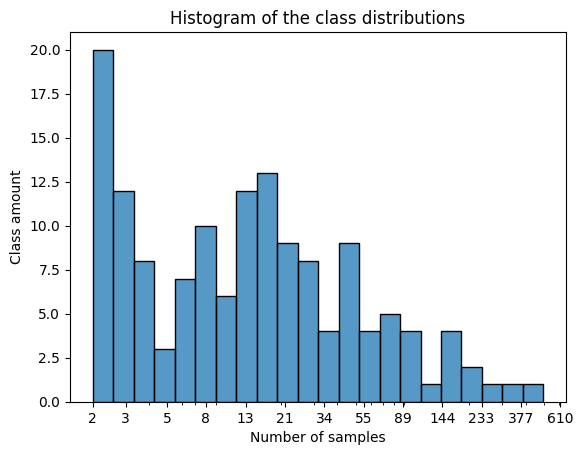
\includegraphics[width=.8\textwidth]{images/histplot.png}
\caption{PLACEHOLDER}
\label{fig:histplot}
\end{figure}  

\section{Evaluation Criteria}
\label{sec:evaluation}

Since a metric learning model yields a distance between two data points (in our case, two documents), we need to define a threshold to declare wether the two data points belong to the same class or not, to calculate how accurate the model is. For this, we use \gls{EER} as metric~\cite{EER}. \gls{EER} is  the point at which the \gls{FAR} and \gls{FRR} are equal. The \gls{EER} is calculated by setting the \gls{FAR} equal to the \gls{FRR} and finding the corresponding threshold at this point~\cite{EER2}. In other words, the \gls{EER} is the value of error rate when the threshold value $\tau_{EER}$ gives 
\begin{equation}
    FAR(\tau_{EER}) = FRR(\tau_{EER}),
\end{equation}
where
\begin{equation} \label{far}
    FAR(\tau) = \frac{\text{Number of false acceptances at threshold~} \tau}{\text{Total number of negative samples}}
\end{equation}
is the probability that a negative sample is incorrectly classified as positive~\cite{EER3}. On the other hand,
\begin{equation} \label{frr}
    FRR(\tau) = \frac{\text{Number of false rejections at threshold~} \tau}{\text{Total number of positive samples}}
\end{equation}
is the probability that a positive sample (e.g., a genuine user) is incorrectly classified as negative.

For each chosen backbone, we we train 10 models: a 5-fold cross-validation for each of the 2 scenarios, \gls{ZSL} and \gls{GZSL}. As shown in Section \ref{sec:method_dataset}, each split follows a fixed validation protocol to ensure consistency. We also evaluate the trained models from each split on the independent test set, to compare them with the \gls{LLM}s. We report the mean \gls{EER} from all splits in a scenario.

\section{Partial Results}
\label{sec:results}

In this section we discuss the current and currentchat results of our research. This section's discussions revolves around Table \ref{tab:res}, where we present the results of every model we trained. The table shows the mean EER value of the cross-validation in both scenarios, as well as the mean performance of each fold on the independent test set. While the ZSL-GZSL scenarios are very influential on the visual models performance, this difference is not relevant on the \gls{LLM} test, as they have not been fine-tuned for the task. While they may have been originally trained with some documents of the RVL-CDIP database, both scenarios are effectively \gls{ZSL}. On Section \ref{sec:visual_models}, we discuss the results of the trained visual models and compare the effects of different backbones in the result. On Section \ref{sec:llm_result}, we compare the results returned by the \glspl{LLM} chosen for this work. Finally, on Section \ref{sec:comparison_result}, we compare both approaches.

% Please add the following required packages to your document preamble:
\begin{table}[ht]
\caption{Comparative performance between different visual backbones and Large Language Models. Following the columns: the architecture name; the architecture edition, if exists; cross-validation over the \gls{ZSL} scenario; cross-validation over the \gls{GZSL} scenario; test performance on the \gls{ZSL} scenario; and test performance over the \gls{GZSL} scenario. Every value is a mean EER (\%) value over the \gls{CV} folds.}
\label{tab:res}
\centering
% Please add the following required packages to your document preamble:
% \usepackage{multirow}
% Please add the following required packages to your document preamble:
% \usepackage{multirow}
\setlength{\tabcolsep}{6pt} % Adjust column spacing
\begin{tabular}{lclcccc}
\toprule
Architecture                            & Edition & Params & \gls{ZSL}    & \gls{GZSL}    & Test \gls{ZSL} & Test \gls{GZSL} \\
\midrule
AlexNet                                 &         &  57M   & 8.92   & 5.45    & 17.33    & 6.31      \\ \midrule
\multirow{4}{*}{VGG}                    & 11      &  129M  & 7.47   & 5.01    & 14.24    & 3.95      \\
                                        & 13      &  129M  & 7.03   & 4.79    & 9.30     & 3.95      \\
                                        & 16      &  134M  & 8.29   & 5.23    & 14.74    & 4.82      \\
                                        & 19      &  139M  & 7.30   & 4.57    & 17.08    & 3.90      \\ \midrule
\multirow{5}{*}{ResNet}                 & 18      &  11M   & 5.03   & 1.54    & 4.98     & 1.51      \\
                                        & 34      &  21M   & 4.32   & 2.10    & 4.13     & 1.53      \\
                                        & 50      &  23M   & 6.90   & 3.39    & 10.34    & 2.21      \\
                                        & 101     &  42M   & 8.20   & 2.72    & 11.31    & 1.98      \\
                                        & 152     &  58M   & 9.44   & 3.38    & 12.70    & 2.39      \\ \midrule
\multirow{2}{*}{MobileNetV3}            & Small   &  1M    & 7.98   & 5.06    & 12.74    & 5.26      \\
                                        & Large   &  4M    & 8.16   & 4.27    & 8.45     & 4.43      \\ \midrule
\multirow{4}{*}{EfficientNet}           & 0       &  4M    & 4.41   & 2.27    & 6.02     & 0.95      \\
                                        & 1       &  6M    & 3.93   & 3.54    & 8.88     & 2.70      \\
                                        & 2       &  7M    & 5.73   & 2.61    & 7.29     & 2.14      \\
                                        & 3       &  10M   & 5.65   & 3.64    & 7.37     & 2.34      \\ \midrule
\multirow{2}{*}{\gls{ViT}}              & Base    &  87M   & 12.43  & 7.97    & 19.72    & 5.19      \\
                                        & Large   &  305M  & 13.16  & 7.57    & 19.88    & 5.26      \\ \midrule
Llama                                &  3.2     &     11B   & --     & --      & 13.95    & 21.90     \\
InternVL                             & 2.5      &   8B     & --     & --      & 8.58     & 10.40     \\
Qwen-VL                              & 2.5       &   7B     & --     & --      & 6.61     & 4.20      \\
GPT 4o mini                                 & 2024-07-18    &   *     & --     & --      & 4.70     & 4.07      \\
GPT 4o                                  & 2024-11-20      &    *    & --     & --      & 2.75     & 1.33      \\ \bottomrule

\end{tabular}
\smallskip
\parbox[t]{\textwidth}{\footnotesize
    * The parameter count of GPT-4o has not been publicly disclosed.}
\end{table}

% \begin{figure}[htbp]
% \centering
% %\isPreprints{\centering}{} % Only used for preprints
% 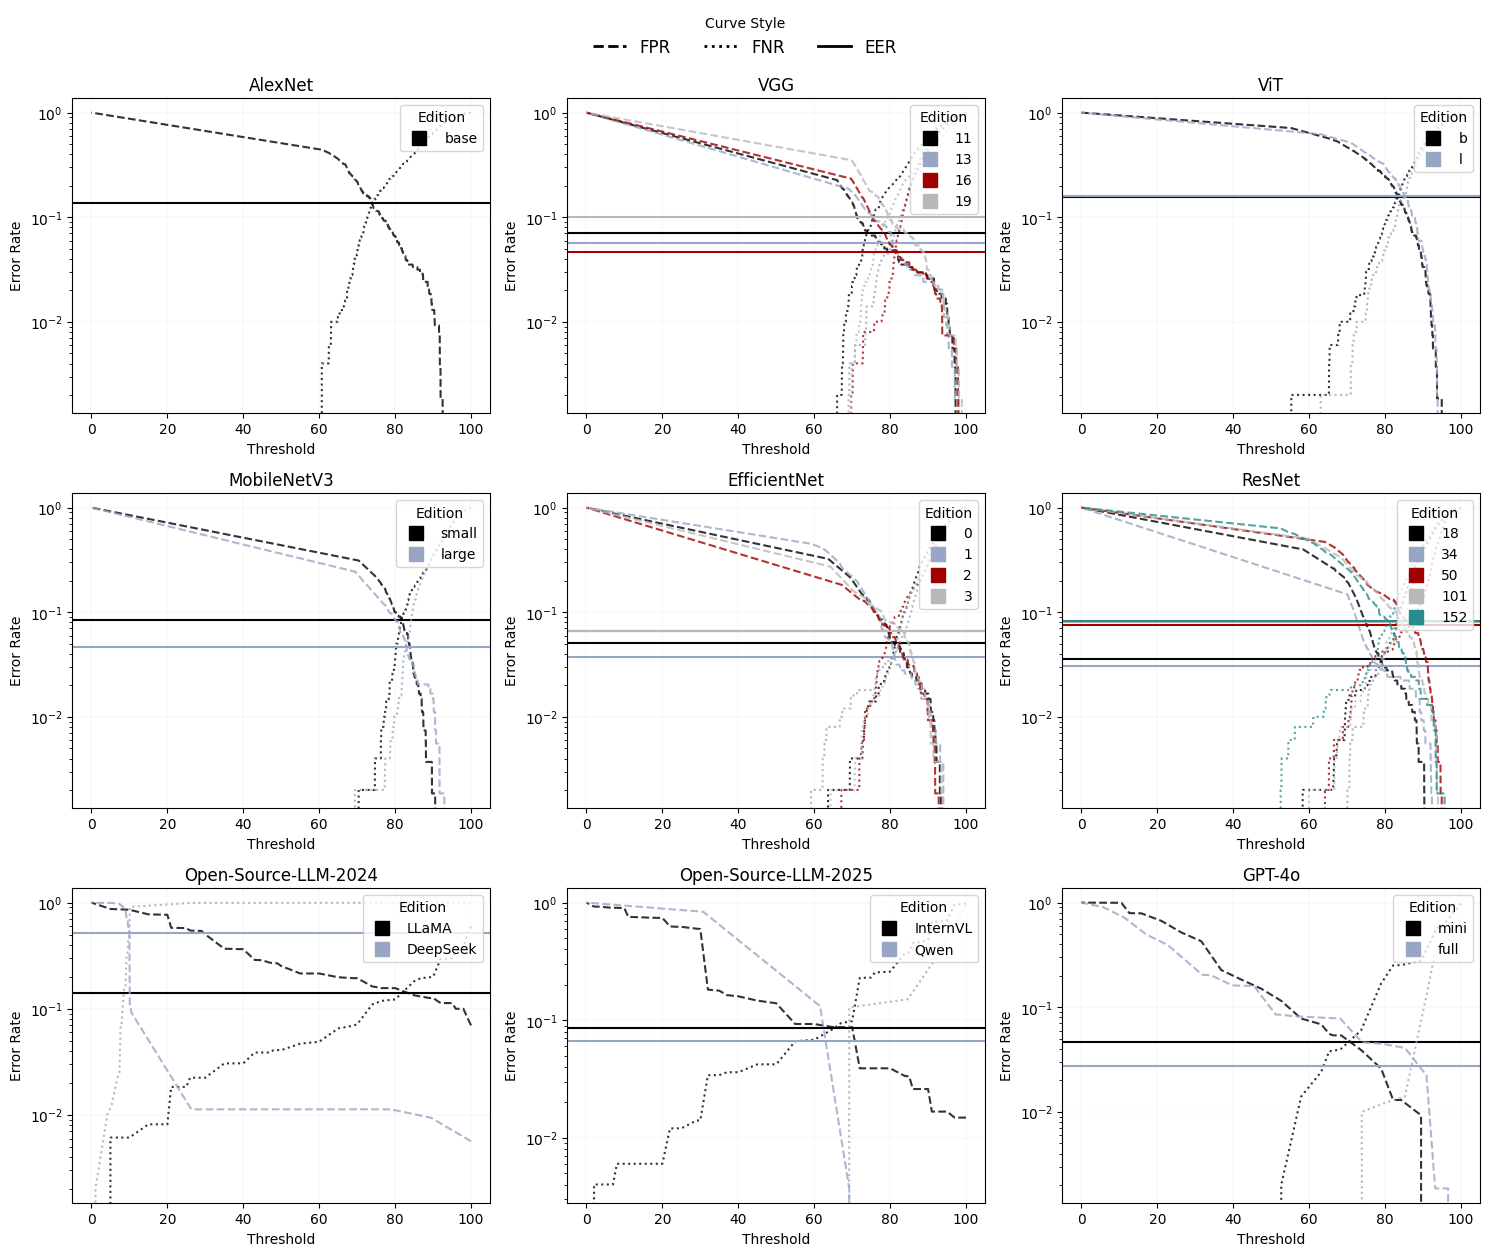
\includegraphics[width=10 cm]{images/ImageFPR_FNR_models_log.png}
% \caption{Models Equal Error Rates (ZSL)\label{fig:eer}}
% \end{figure}  

\subsection{Visual Models}
\label{sec:visual_models}

Among visual models, smaller and more cost-efficient architectures outperformed larger ones. This trend is evident in different ResNet variants: ResNet-18 and ResNet-34 showed strong performance, while larger versions (ResNet-50, ResNet-101, and ResNet-152) performed progressively worse. We also observed that Vision Transformer (ViT), despite excelling on datasets like ImageNet \cite{imagenet}, was the worst-performing model in this task. We can see in Figure \ref{fig:tsne} that, while none of the class separations are perfect, ResNet-18 and EfficientNet-b0 have a better inter-class separation, if compared against ViT-b and ViT-l. These larger models overfitted to the training data, with some reaching 0\% train error in certain epochs while maintaining a high validation error. The most likely cause of this behavior is the dataset size—LA-CDIP contains only 4,993 documents, with approximately two-thirds used for training in each fold. However, techniques such as tuple mining and data augmentation could help mitigate this effect by increasing the diversity of training samples and improving feature learning. The overall best models are the ResNet-34, and EfficientNet-0 and 1. They offer a balance in size, achieving a good generalization of the problem while also learning the intricacies the task demands.

% \begin{figure}[htbp]
% \centering
% %\isPreprints{\centering}{} % Only used for preprints
% 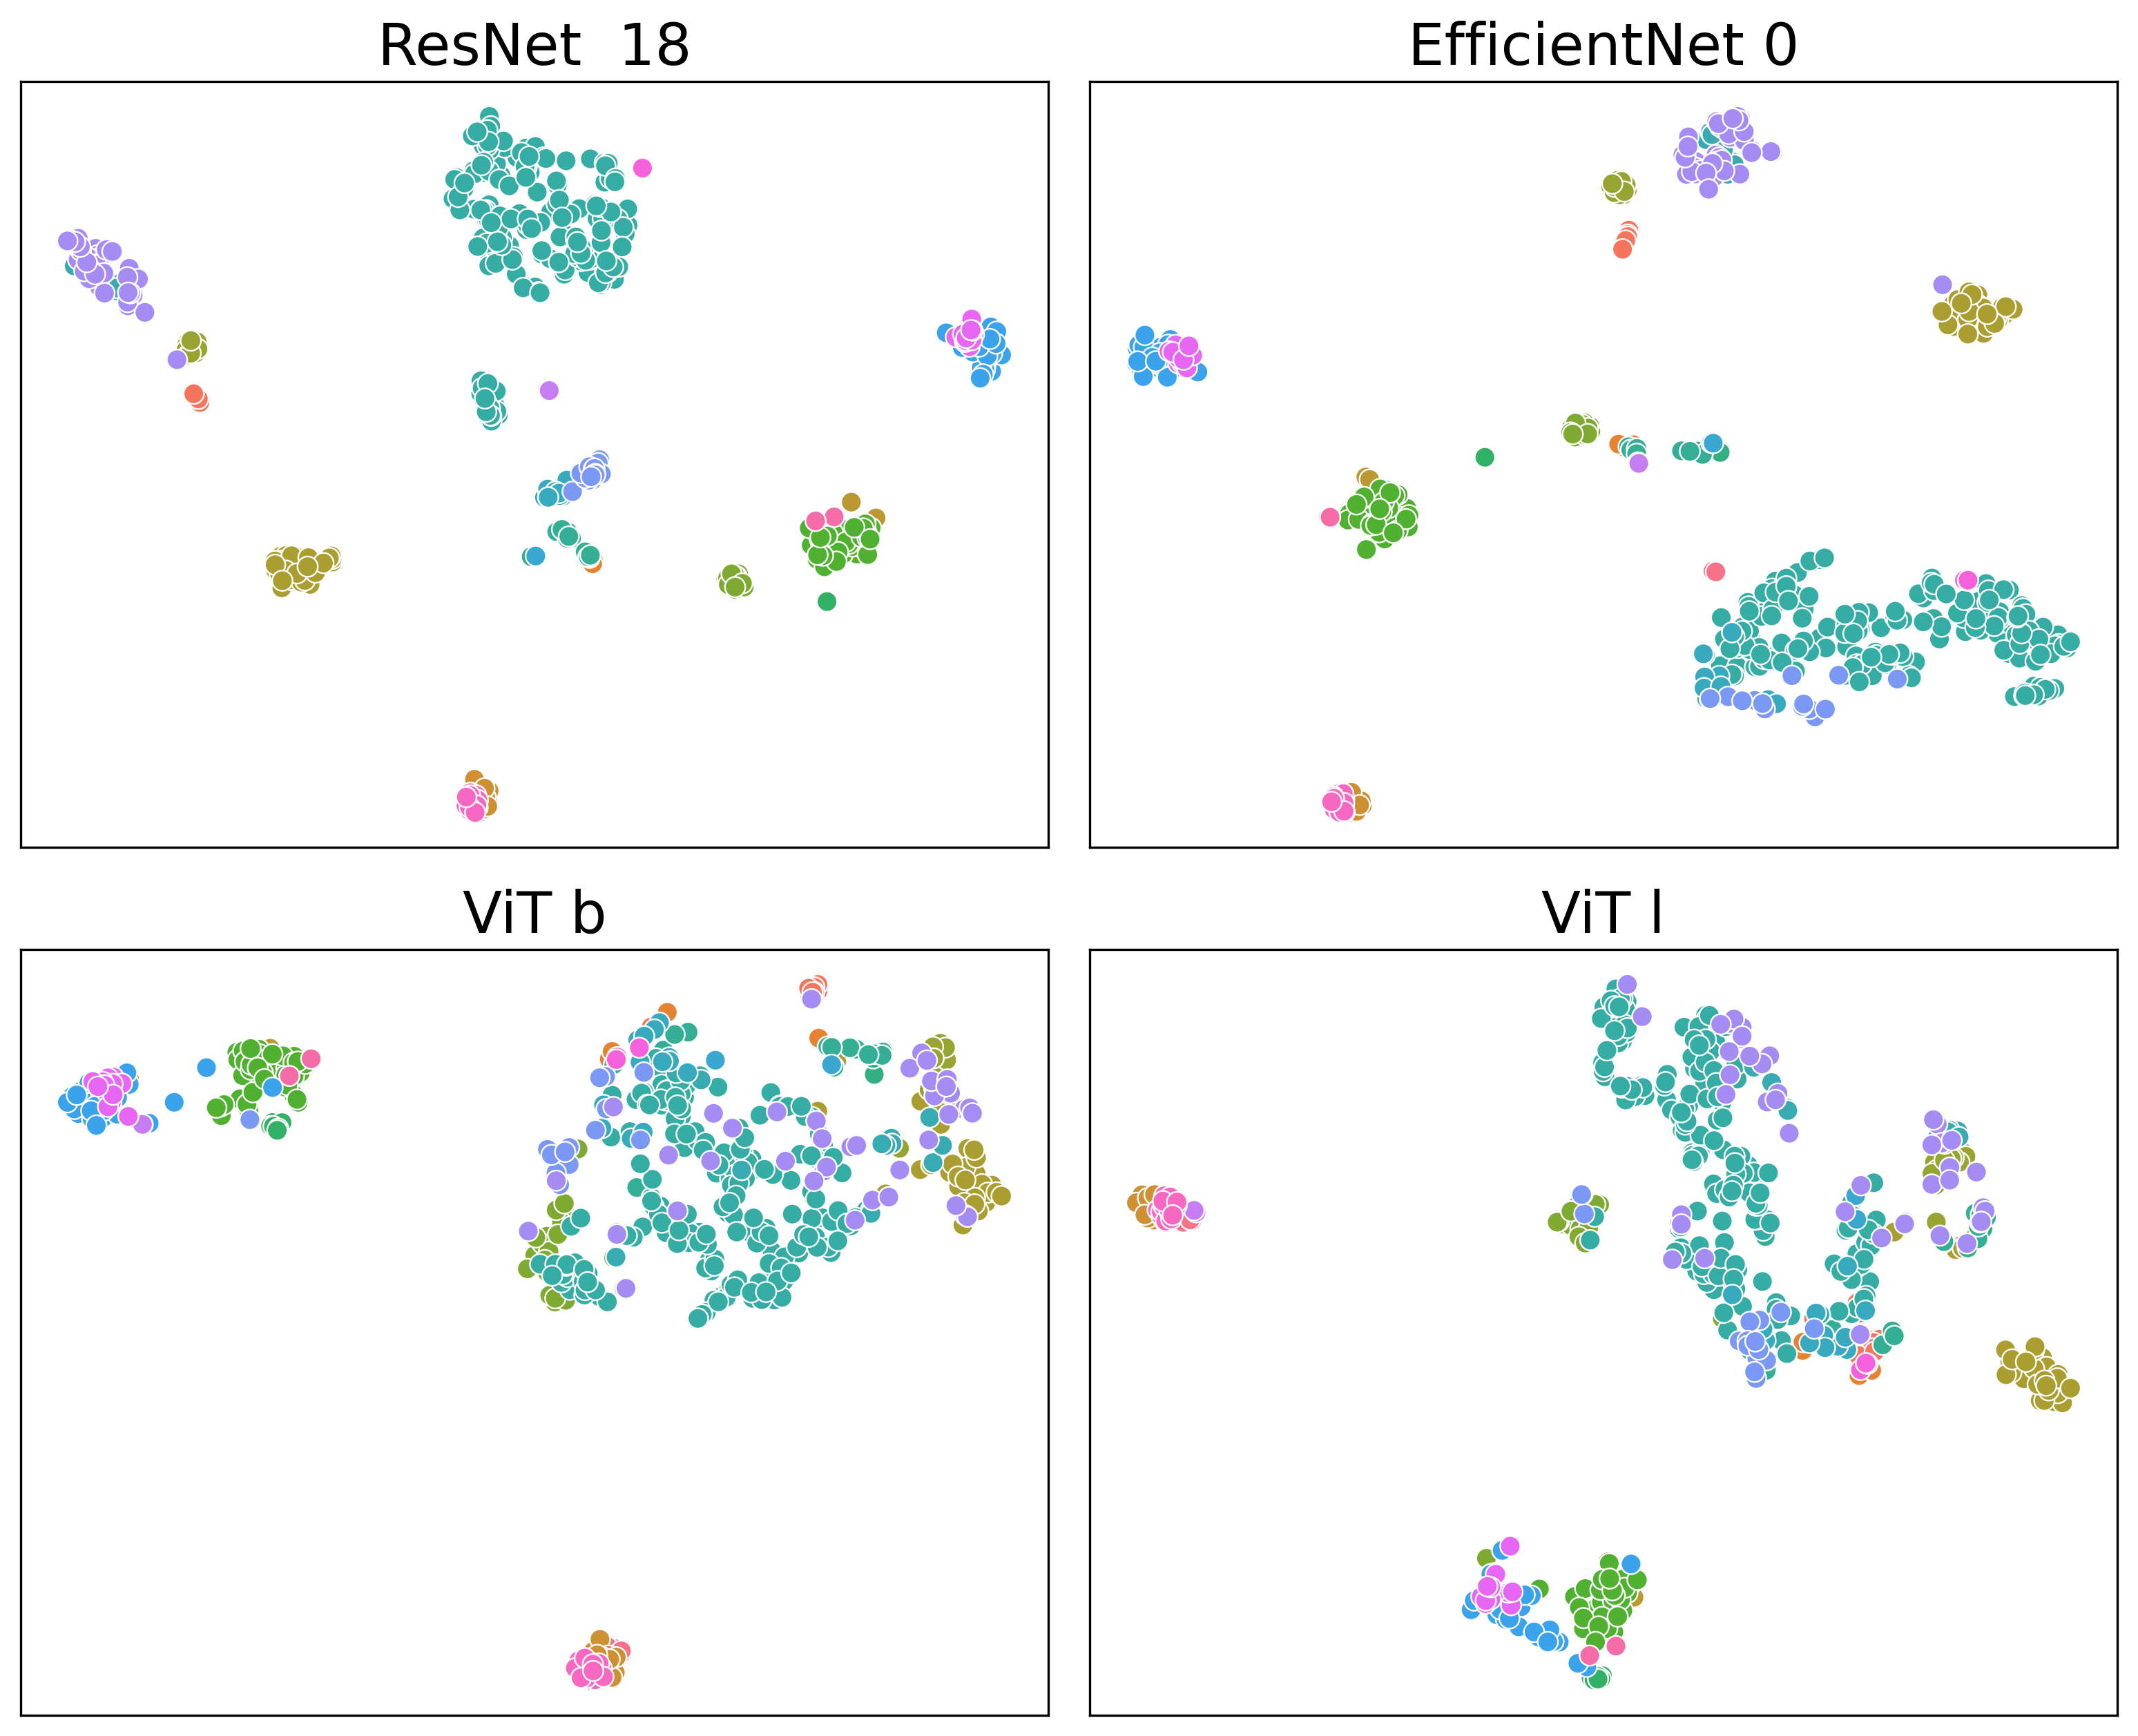
\includegraphics[width=10 cm]{images/TSNE.png}
% \caption{TSNE visualization of the Test ZSL scenario. These models have been trained on the same cross-validation fold.\label{fig:tsne}}
% \end{figure}  

\begin{figure}[htbp]
    \centering
    \begin{minipage}{0.4\linewidth}
        \centering
        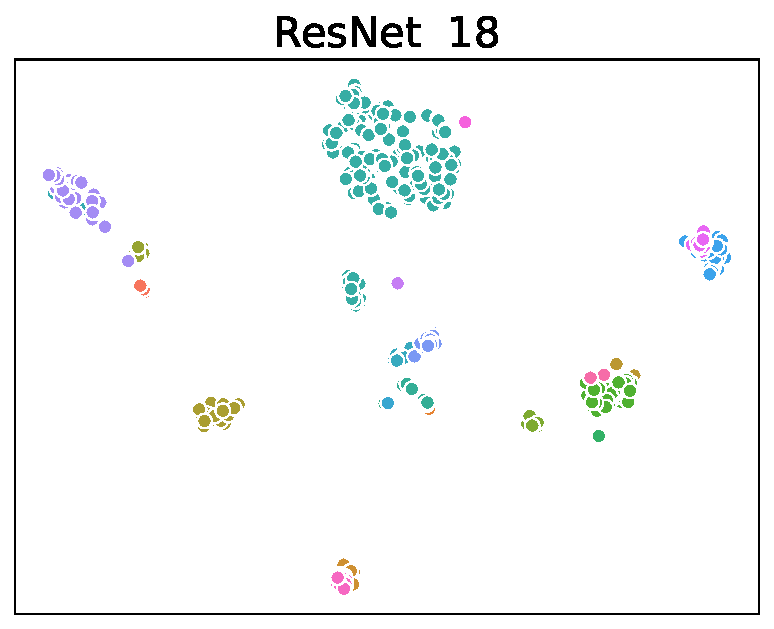
\includegraphics[width=\linewidth]{images/ResNet.csv_18_0.pdf}
        % \caption{Similar Comparison}
    \end{minipage}
    \begin{minipage}{0.4\linewidth}
        \centering
        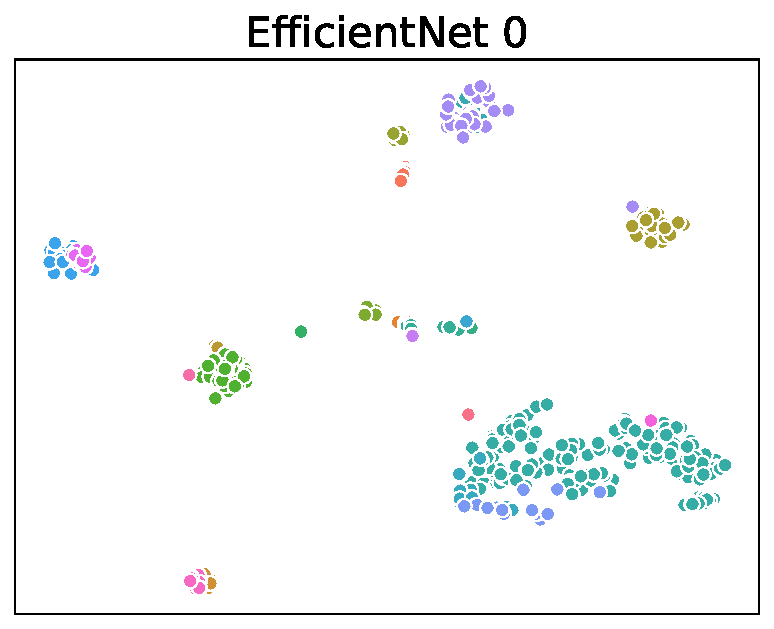
\includegraphics[width=\linewidth]{images/EfficientNet.csv_0_0.pdf}
        % \caption{Different Comparison}
    \end{minipage}
    \begin{minipage}{0.4\linewidth}
        \centering
        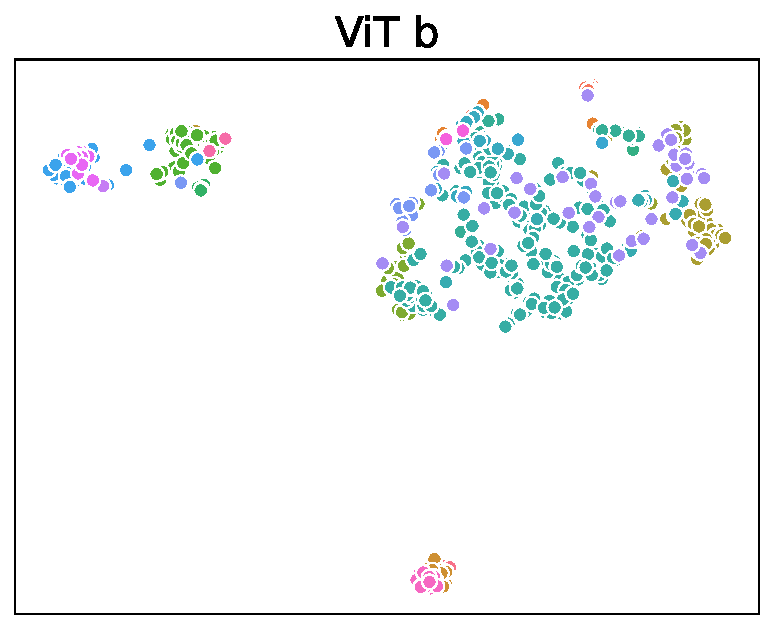
\includegraphics[width=\linewidth]{images/ViT.csv_b_0.pdf}
        % \caption{Different Comparison}
    \end{minipage}
    \begin{minipage}{0.4\linewidth}
        \centering
        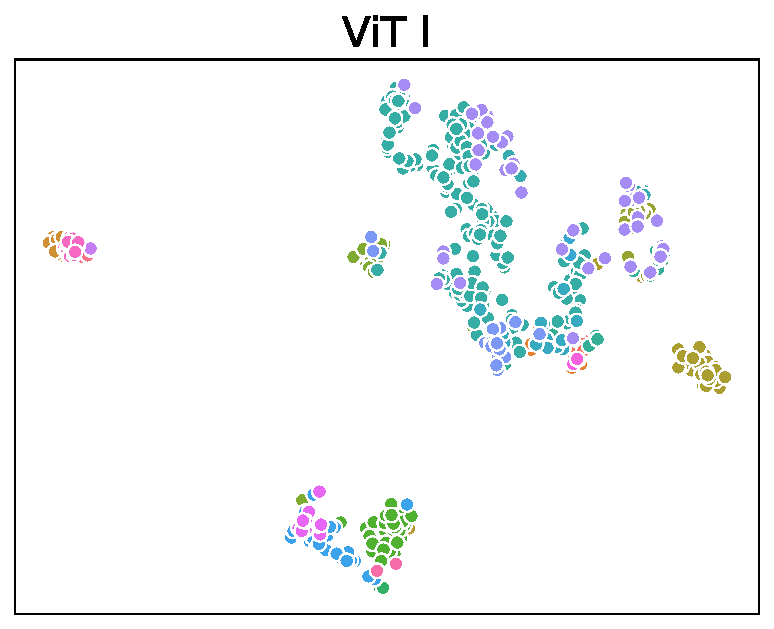
\includegraphics[width=\linewidth]{images/ViT.csv_l_0.pdf}
        % \caption{Different Comparison}
    \end{minipage}
    \caption{TSNE visualization of the Test ZSL scenario. These models have been trained on the same cross-validation fold.\label{fig:tsne}}
\end{figure}

Comparing the \gls{ZSL} and the \gls{GZSL} results, we can see that the \gls{GZSL} consistently gives better results. This is expected, since half of the validation set on each fold is composed of classes seen in training. The biggest discrepancies between the two modalities can be seen in the largest models, where the overfitting damage is mitigated by the easier scenario. Even so, the best performance on the \gls{GZSL} scenario is usually connected with a good performance on the \gls{ZSL} scenario.

In the test scenarios, the reported values represent the mean performance across all folds, evaluated on the same set. Since this is a Zero-shot data split, there is inherently a high variance over the different splits, since they test on entirely different patterns each fold. We observe that, by chance, the \gls{ZSL} test split is more challenging than average, resulting in higher error rates for most models relative to the mean cross-validation error rate. The test \gls{GZSL} scenario follows the opposite reasoning.

\subsection{Large Language Models}
\label{sec:llm_result}

As a result, all models were tested under similar conditions, however, further performance improvements could be achieved through refined prompt engineering.. Therefore, the results presented should not be considered as definitive comparisons of the models' capabilities but rather a baseline for assessing the viability of our proposed method. Despite these limitations, \gls{LLM} results align with existing benchmarks for document understanding tasks for these models. 

As shown in Table~\ref{tab:res}, GPT-4o exhibited the best overall performance, achieving the lowest error rates in both the \gls{ZSL} and \gls{GZSL} scenarios. The GPT-4o-mini variant performed similarly but showed slightly lower accuracy, reflecting its trade-off between efficiency and capability.

Additionally, Llama 3.2 Vision faced challenges in handling multiple document inputs, requiring images to be combined into a single input before processing. This limitation impacted its ability to directly compare layouts across distinct documents, differentiating its approach from the other evaluated models.

InternVL 2.5 and Qwen2.5-VL emerged as open-source alternatives for  \gls{ZSL} \gls{VDM}. Notably, the QwenVL 7B model reached performance levels close to those of GPT-4o mini, further highlighting the efficiency of these compact architectures.

Since the \glspl{LLM} have not been fine-tuned with the training data, the only difference between the \gls{ZSL} and \gls{GZSL} scenarios is the number of classes to compare: \gls{ZSL} has exactly $\frac{1}{6}$ of the classes and \gls{GZSL} can have every class, making \gls{GZSL} a more complete test. Surprisingly, the two models performed with different trends between both scenarios: InternVL was better at the \gls{ZSL} split, and GPT better at the \gls{GZSL} split.

\subsection{Comparison}
\label{sec:comparison_result}

Given that \gls{GZSL} is an advantageous scenario for vision models—since they have been trained on half of the classes—while \glspl{LLM} have not been fine-tuned for this task, both settings effectively serve as pure zero-shot evaluations. Therefore, the comparison was conducted in the \gls{ZSL} scenario.

When compared to most \glspl{LLM}, \gls{LA-ZSL} enabled visual models to handle \gls{ZSL} \gls{VDM} while maintaining a significantly lower parameter count. This relationship between performance and model efficiency is illustrated in Figure~\ref{fig:performance}.

\begin{figure}[htbp]
\centering
%\isPreprints{\centering}{} % Only used for preprints
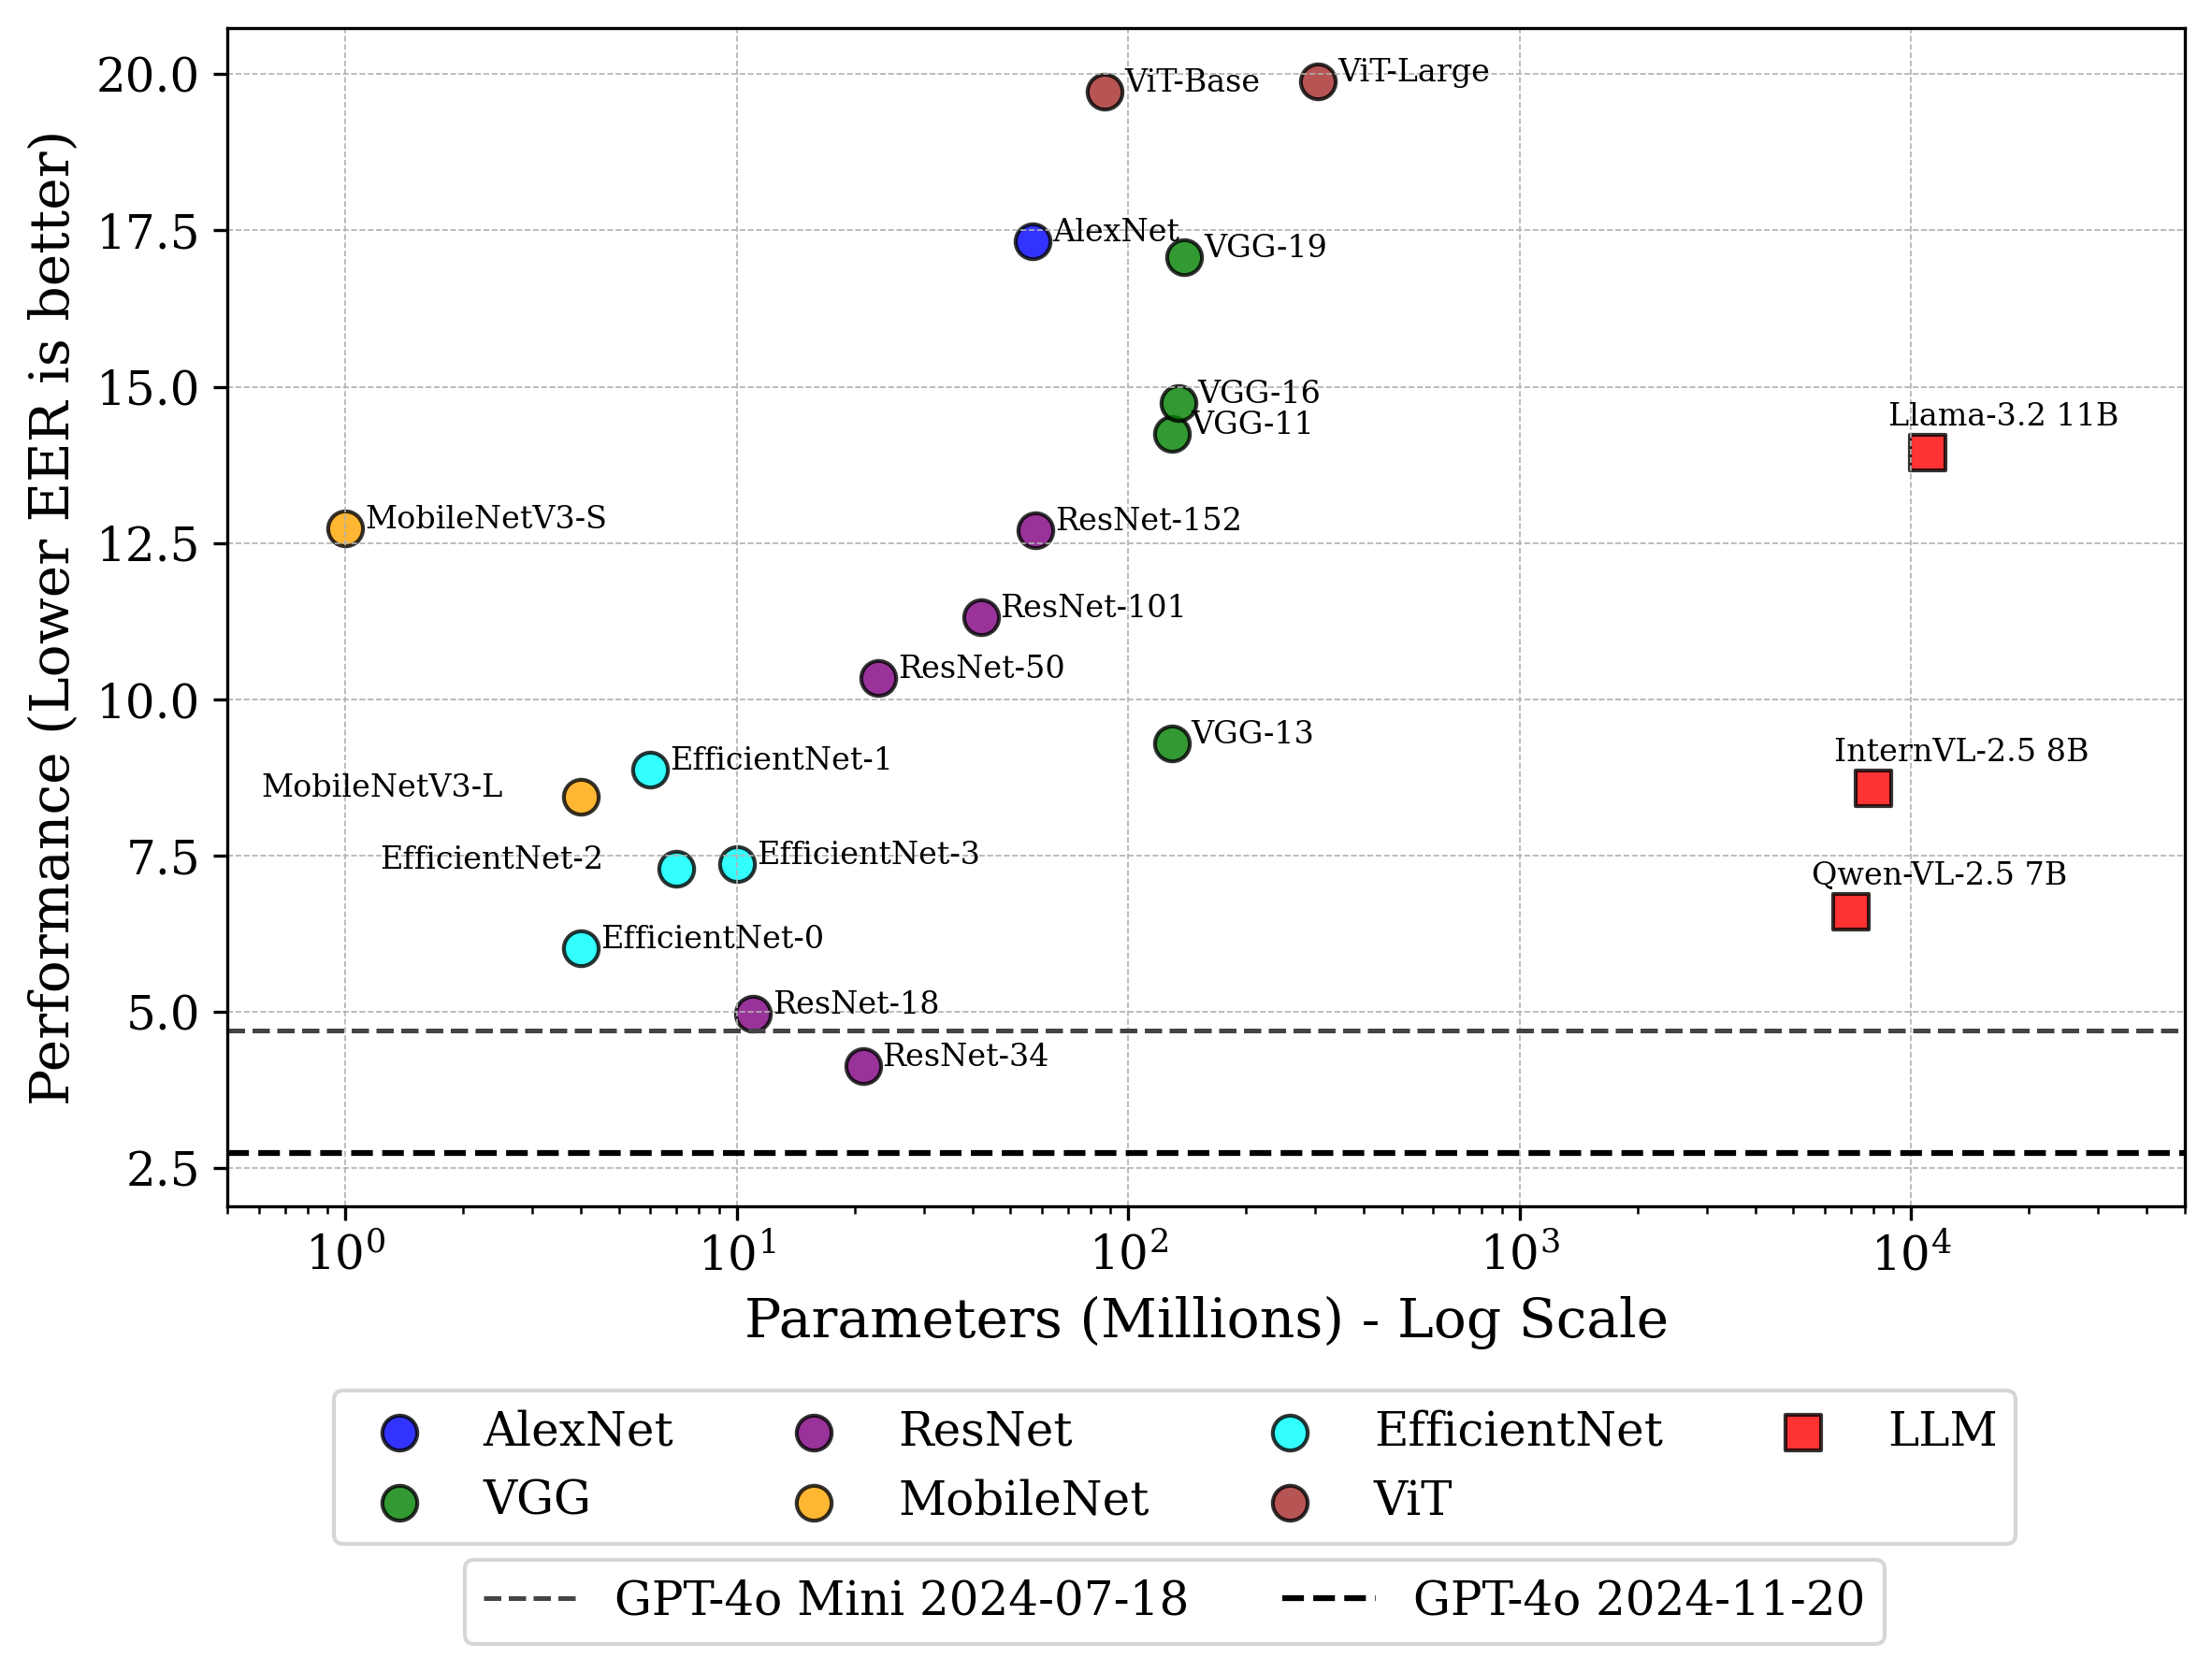
\includegraphics[width=1\linewidth]{images/performance_vs_parameters.png}
\caption{Performance vs Parameters (ZSL)\label{fig:performance}}
\end{figure}  

The results highlight a trade-off between model complexity and effectiveness. Smaller visual backbones, such as ResNet-18 and EfficientNet-0, achieve competitive performance while using significantly fewer parameters than large multimodal models. Notably, ResNet-18 and ResNet-34 exhibit lower error rates than several larger architectures, reinforcing the efficiency of lightweight vision models in document matching tasks.
